\documentclass[%
 aapm,
 mph,%
 amsmath,amssymb,
%preprint,%
 reprint,%
%author-year,%
%author-numerical,%
]{revtex4-2}

\usepackage{graphicx}% Include figure files
\usepackage{dcolumn}% Align table columns on decimal point
\usepackage{bm}% bold math

\usepackage{mathtools}
\usepackage[mathlines]{lineno}% Enable numbering of text and display math

\begin{document}

\preprint{AAPM/123-QED}

\title[Ion transport in a retarding field energy analyzer]{ERIKA: Emulating Retarding-field-energy-analyzer Ion Kinetic-transport in Argon-gas}

\author{Felipe Soberon}
 \altaffiliation{Impedans Ltd.}
 \email{felipe.soberon@impedans.com}
 \homepage{http://www.impedans.com}

\date{\today}

\begin{abstract}
This document reports a one-dimensional simulation of the transport of argon ions across a plasma sheath and through a
retarding field energy analyzer (RFEA). The simulation can model DC and AC sheaths. The DC sheath is modeled using Child Law
and the AC sheath using the analytical solution of a radio-frequency capacitive sheath by M. A. Lieberman. The model includes
elastic and charge exchange ion collisions with background Argon gas. 
\end{abstract}

\keywords{Plasma sheath, Child Law, RF sheath, Charge exchange collision, Retarding Field Energy Analyzer (RFEA)}
\maketitle

\section{\label{Introduction}Introduction}

Retarding field analyzers are employed to assess the energy distribution of ions impinging on a surface. Ions acquire considerable kinetic energy as a result of the high voltage across the plasma sheath. This energy distribution is valuable in various applications, such as space propulsion equipment. In other contexts, such as the manufacturing of semiconductor devices, plasma etching equipment, or plasma deposition, the ion energy serves as a parameter that can influence the etch rate, the profile of the process, or the deposition rate.

RFEA devices can be designed as an array of thin grids tightly packed together, with a series of voltages applied to these grids. The primary purpose of this configuration is to select ions based on their energy and to eliminate the detection of electrons originating from the plasma discharge or secondary electrons emitted by the RFEA following ion impact. 

The operational range of RFEA devices is limited by several factors, including background gas pressure, fast electrons from the plasma, secondary electrons emitted within the RFEA, ionization occurring inside the RFEA, the distance between RFEA grids, and field distortion within the RFEA caused by space charge.

To assess the impact of any of the factors mentioned above, a computer simulation of a plasma sheath and RFEA grid would enable one to explore these factors individually or in combination.

Here we report a one-dimensional model of a plasma sheath and RFEA device. 
 
\section{\label{Simulation}Simulation Description}
In this section we provide details of the model. Subsection \ref{SpacePotentialAndField} describe how the space potential and electric field are calculated including the plasma sheath and in the RFEA region. Subsection \ref{IonTrajectory} describe the method to integrate the ion trajectories under the effect of the fields decribed in subsection \ref{SpacePotentialAndField}. Subsection \ref{IonCollision} describes the method to simulate ion collisions with the background gas. 

\subsection{\label{SpacePotentialAndField}Space Potential and Electric Field}
The space potential and electric field are calculated in two regions: the RFEA region, and the plasma sheath. The model is one-dimensional, therefore only space potential and electric field in the z-axis is calculated in these regions. In this geometry, the RFEA is located at $z \leq 0$ and its extension in the negative direction of the z-axis depends on the spaces between the grids and the collector; subsection \ref{RFEA}. The plasma sheath starts at $z=0$ and extends to the plasma, which is located at some $z_\text{plasma} > 0$. The location of the plasma sheath boundary edge depends on the plasma sheath model and is further described in subsection \ref{SheathModel}.   

\subsubsection{\label{RFEA}Retarding Field Energy Analyzer}
The RFEA modeled includes the standard four grids and collector plate~\cite{Hutchinson1987}. These are identified as G$_0$, G$_1$, G$_2$, G$_3$, C. The first grid, G$_0$, faces the plasma and is at the same potential as the electrode that bounds the plasma discharge. In this model, the voltage of G$_0$ is set to zero. The second grid, G$_1$ is typically biased negative respect to G$_0$ to repel electrons from the plasma discharge. The model does not include electrons, however, this grid is included to simulate the electric field that affects the motion of ions between G$_0$ and G$_1$. The third grid, G$_2$, is used to discriminate ions by setting the voltage of G$_2$ positive relative to G$_0$. The voltage of G$_2$ is typically swept from zero to a large voltage to limit the ion current to the collector and generate the RFEA characteristic voltage-current curve. The fourth grid, G$_3$, is used to repel secondary electrons that may be emitted by the collector due to ion impact. This grid is usually biased slightly negative relative to the voltage applied to the collector. Again, the model does not include electrons, however, it is included to simulate the electric field between G$_3$ and the collector that afect the ion trajectories. Finally, the last electrode in the RFEA is the collector, C, which is biased somewhat negative relative to the first grid, G$_0$.

The model assumes that the grids and non-dimensional; i.e. zero thickenss. This differs from actual RFEA devices where the grids are usually 40~$\mu$m thick (reference some publication by Impedans). Consequently, the model also neglects any lensing effects of non-zero thick grids~\cite{vandeVen2018,Buiter2018}. The distance between grids and the collector are defined in the model as multiples of 100~$\mu$m. In actual RFEA devices the grids are physically separated by sheets of Mica, 100$\mu$m thick each sheet. The arrangement of grids and spacers is known as the RFEA button stack. For instance, the standard RFEA button stack of a commercial device comprises two spacers between G$_0$ and G$_1$, three spacers between G$_1$ and G$_2$, three spacers between G$_2$ and G$_3$, and two spacers between G$_3$ and the collector C (reference impedans website Semion). This arrangement is therefore known as a 2332 button stack. The model can simulate the RFEA with any combination of button stack arragements expressed as multiples of the basic spacer. 

Besides lensing effects, not included in this model, actual grids are not entirely transparent and a fraction of ions moving through the RFEA are collected by the grids. The transparency of the grids depends on the ion energy and may vary due to the lensing effect. While the model presented here does not simulate these effects it includes a simple transparency factor setting. The user can set this number to any value from 0 to 100\%. The transparency setting is common to all grids; i.e., the transparency of grids cannot be set individually.     

The space potential between grids is calculated by linear interpolation. Similarly, the electric field between grids is calculated as the potential difference between each grid pair divided by the distance. Figure~\ref{fig:DCpotentialField} shows the space potential and electric field in the RFEA for grid voltage settings G$_0$=0, G$_1$=-60, G$_2$=250, G$_3$=-70, and C=-60~V. The location of the grids and collector is indicated with vertical dashed lines. 


\subsubsection{\label{SheathModel}Sheath Model}
The space potential and electric field in the sheath region of the plasma is determined from the Child Law sheath model for direct-current sheath~\cite{Lieberman2005}, and from the analytical solution of capacitive radio-frequency sheath for alternate-current sheath~\cite{Lieberman1988}. These two solutions are collisionless and therefore not valid when the background pressure of neutral argon is high. Therefore this limits the model simulating pressure parameter. Nonetheless, RFEAs are most useful in low pressure plasmas where the ion energy gain is not impeded by frequent collisions and we shall limit simulations to a maximum pressure of 10~Pa (75~mTorr, 100~$\mu$bar).  

For the DC case, the Child Law sheath size is calculated 
\begin{equation}
s_\text{Child Law} = \frac{\sqrt{2}}{3} \lambda_D \left( \frac{2 V_0}{T_e} \right)^{3/4}
\end{equation}
Where $\lambda_D$ is the Debye length
\begin{equation}
\lambda_D = \sqrt{ \frac{\epsilon_0 T_e}{e n_s} }
\end{equation}
Where $T_e$ is the electron temperature (in eV), $\epsilon_0$ is vacuum permittivity (in Farads/metre), $e$ is the basic electric charge (in Coulomb), and $n_s$ is the plasma density at the sheath edge (in m$^{-3}$).

The voltage in the Child Law sheath is given by
\begin{equation}
V_\text{Child Law}(z) = V_0 \left( 1 -  \left( 1 -\frac{z}{s_\text{Child Law}} \right)^{4/3} \right)
\end{equation}
Where the position variable, $z$, is given in metres, and where $V_0$ is the voltage of the plasma sheath edge relative to the bounding electrode at $z=0$. The voltage is null at $z=0$ and $V_0$ at $z=s_\text{Child Law}$. The plasma potential is positive relative to the electrode, therefore $V_0$ is positive.

The electric field (in V/m) is given by
\begin{equation}
E_\text{Child Law}(z) = -\frac{4}{3} \frac{V_0}{s_\text{Child Law}} \left( 1 - \frac{z}{s_\text{Child Law}}  \right)^{1/3}
\end{equation}
Note the field is null at $z=s_\text{Child Law}$ and negative otherwise in the sheath region. 

Figure~\ref{fig:DCpotentialField} shows the space potential and electric field for the DC sheath solution with a voltage across the sheath of 1000~V and plasma density $n_s = 10^{16}$~m$^{-3}$. Note that even for a small voltage at the discriminator grid G$_2$ (relative to the plasma potential) the electric fields within the RFEA are much higher than the electic field across the sheath due to the proximity between grids; i.e., ions experience substantially higher forces within the RFEA. 

\begin{figure}[htbp]
\centering
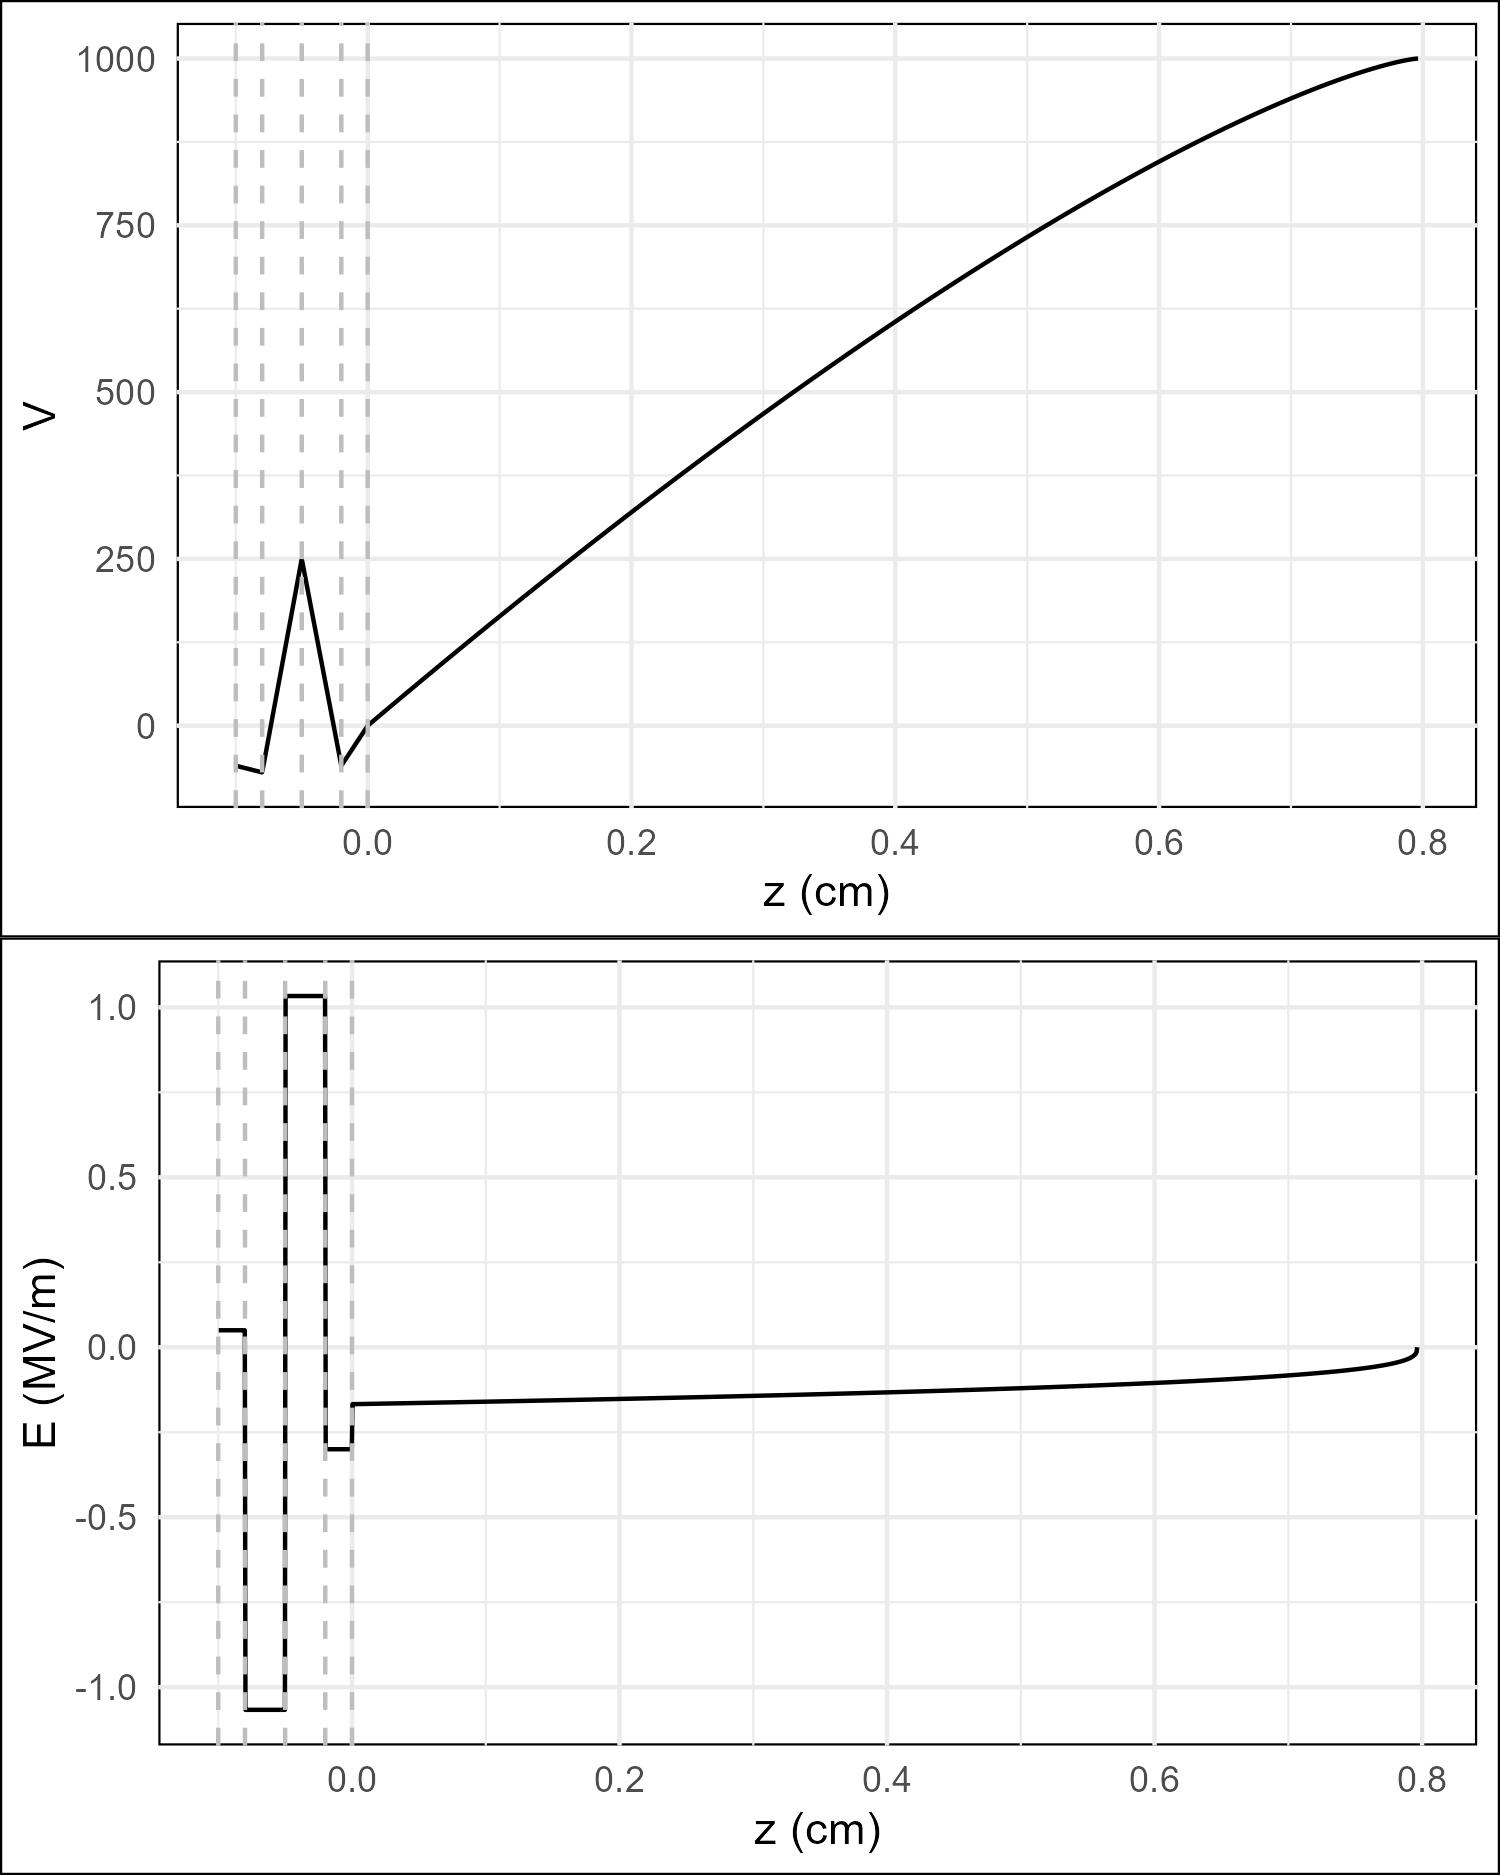
\includegraphics[width=0.45\textwidth]{Figures/VEz2DC1kVStack2332.jpeg}
\caption{Space potential across a plasma sheath and RFEA grid stack (top) and corresponding electric field (bottom) for DC plasma sheath with a voltage across the sheath of 1000~V. The edge of the plasma sheath and plasma is at $z=0.8$~cm. The RFEA is located at $z\le0$; with the plasma facing grid (G$_0$) at $z=0$. The location of the RFEA grids and collector are indicated by vertical dashed lines.}
\label{fig:DCpotentialField}
\end{figure}



The space potential and electric field for the AC sheath are calculated using the capacitive sheath solution of Lieberman~\cite{Lieberman1988}. The sheath edge of the capacitive radio-frequency discharge changes through the cycle, from collapsing when the voltage across the sheath drops to its minimum to full expansion when the voltage is maximum. The size of the sheath is given by, 
\begin{eqnarray}
s(\phi) &=& s_0 ( 1 - \cos(\phi) + \frac{H}{8} \{ \frac32 \sin(\phi)  + \frac{11}{18} \sin(3 \phi) \nonumber \\ 
        & & - 3 \phi \cos(\phi)  - \frac13 \phi \cos(3 \phi)  \} )
\end{eqnarray}
With $\phi = \omega t$ ($\omega = 2 \pi f$) and $f$ the radio-frequency. The value of $s(t)$ is limited to $\phi$ in the range from 0 ($t=0$) to $\pi$ ($t=T/2$; where $T=1/f$ is the radio-frequency cycle period). The size of the sheath at $t=0$ is zero and its maximum size at $s(t=T/2) = s_m$. The $s(t)$ function can be evaluated at any time value via the following 
\begin{eqnarray}
s(t)    &=& \text{abs}(s(\omega \tau(t))) \\
\tau(t) &=& \text{remainder}\left(\frac{t}{T}+\frac12\right) - \frac{T}{2} 
\end{eqnarray}
The parameter $s_0$ is given by 
\begin{equation}
s_0 = \frac{J}{e n_s \omega}
\end{equation}
$J$ is the total current through the plasma discharge (mainly displacement current in the sheaths and conduction current in the plasma bulk). The current can be calculated from the plasma density at the sheath edge ($n_s$) and the maximum voltage across the sheath ($V_0$)
\begin{equation}
J = \frac25 \omega \sqrt{\frac65} \sqrt{e n_s \epsilon_0 (\sqrt{576+125 V_0}-24)}
\end{equation}
The $H$ parameter is given by
\begin{equation}
H = \frac1{\pi} \frac{s_0^2}{\lambda_D^2}
\end{equation}

The electric field in the z-direction is given by 
\begin{equation}
E_{AC}(z,t) = \frac{J}{\epsilon_0 \omega} \left \{ \cos(\omega t) - \cos(\phi(s_m - z)) \right \} 
\end{equation}
If $s(t)<s_m-z$, otherwise the electric field is zero. Note that the function $\phi(s)$ is the inverse of the sheath size $s(\phi)$, that it does not have an analytical solution, and that it is numerically solved in the computer code. 64 pairs $(s(\phi), \phi)$ for $\phi$ from 0 to $\pi$ in steps of $\pi/64$ are generated. The value of $\phi$ for a given $s$ is detemined by linear interpolation of the two nearest pairs.   

Finally, the space potential for the capacitive radio-frequency sheath is given by the integral
\begin{equation}
V_{AC}(z,t) = \int_{0}^{z} E_{AC}(\xi, t) d\xi
\end{equation}
With $z$ in the range from $z=0$ to $z=s_m$. The field is numerically integrated.  

The space potential and electric field for the AC sheath solution are shown in Fig.~\ref{fig:ACpotentialField}. The curves plotted show both results at times 0, T/4 and T/2. Note that at T/2 the voltage across the sheath is null and there is no electric field acting on the ions. This modulation affects the ion motion; this is illustrated in the next subsection. 

\begin{figure}[htbp]
\centering
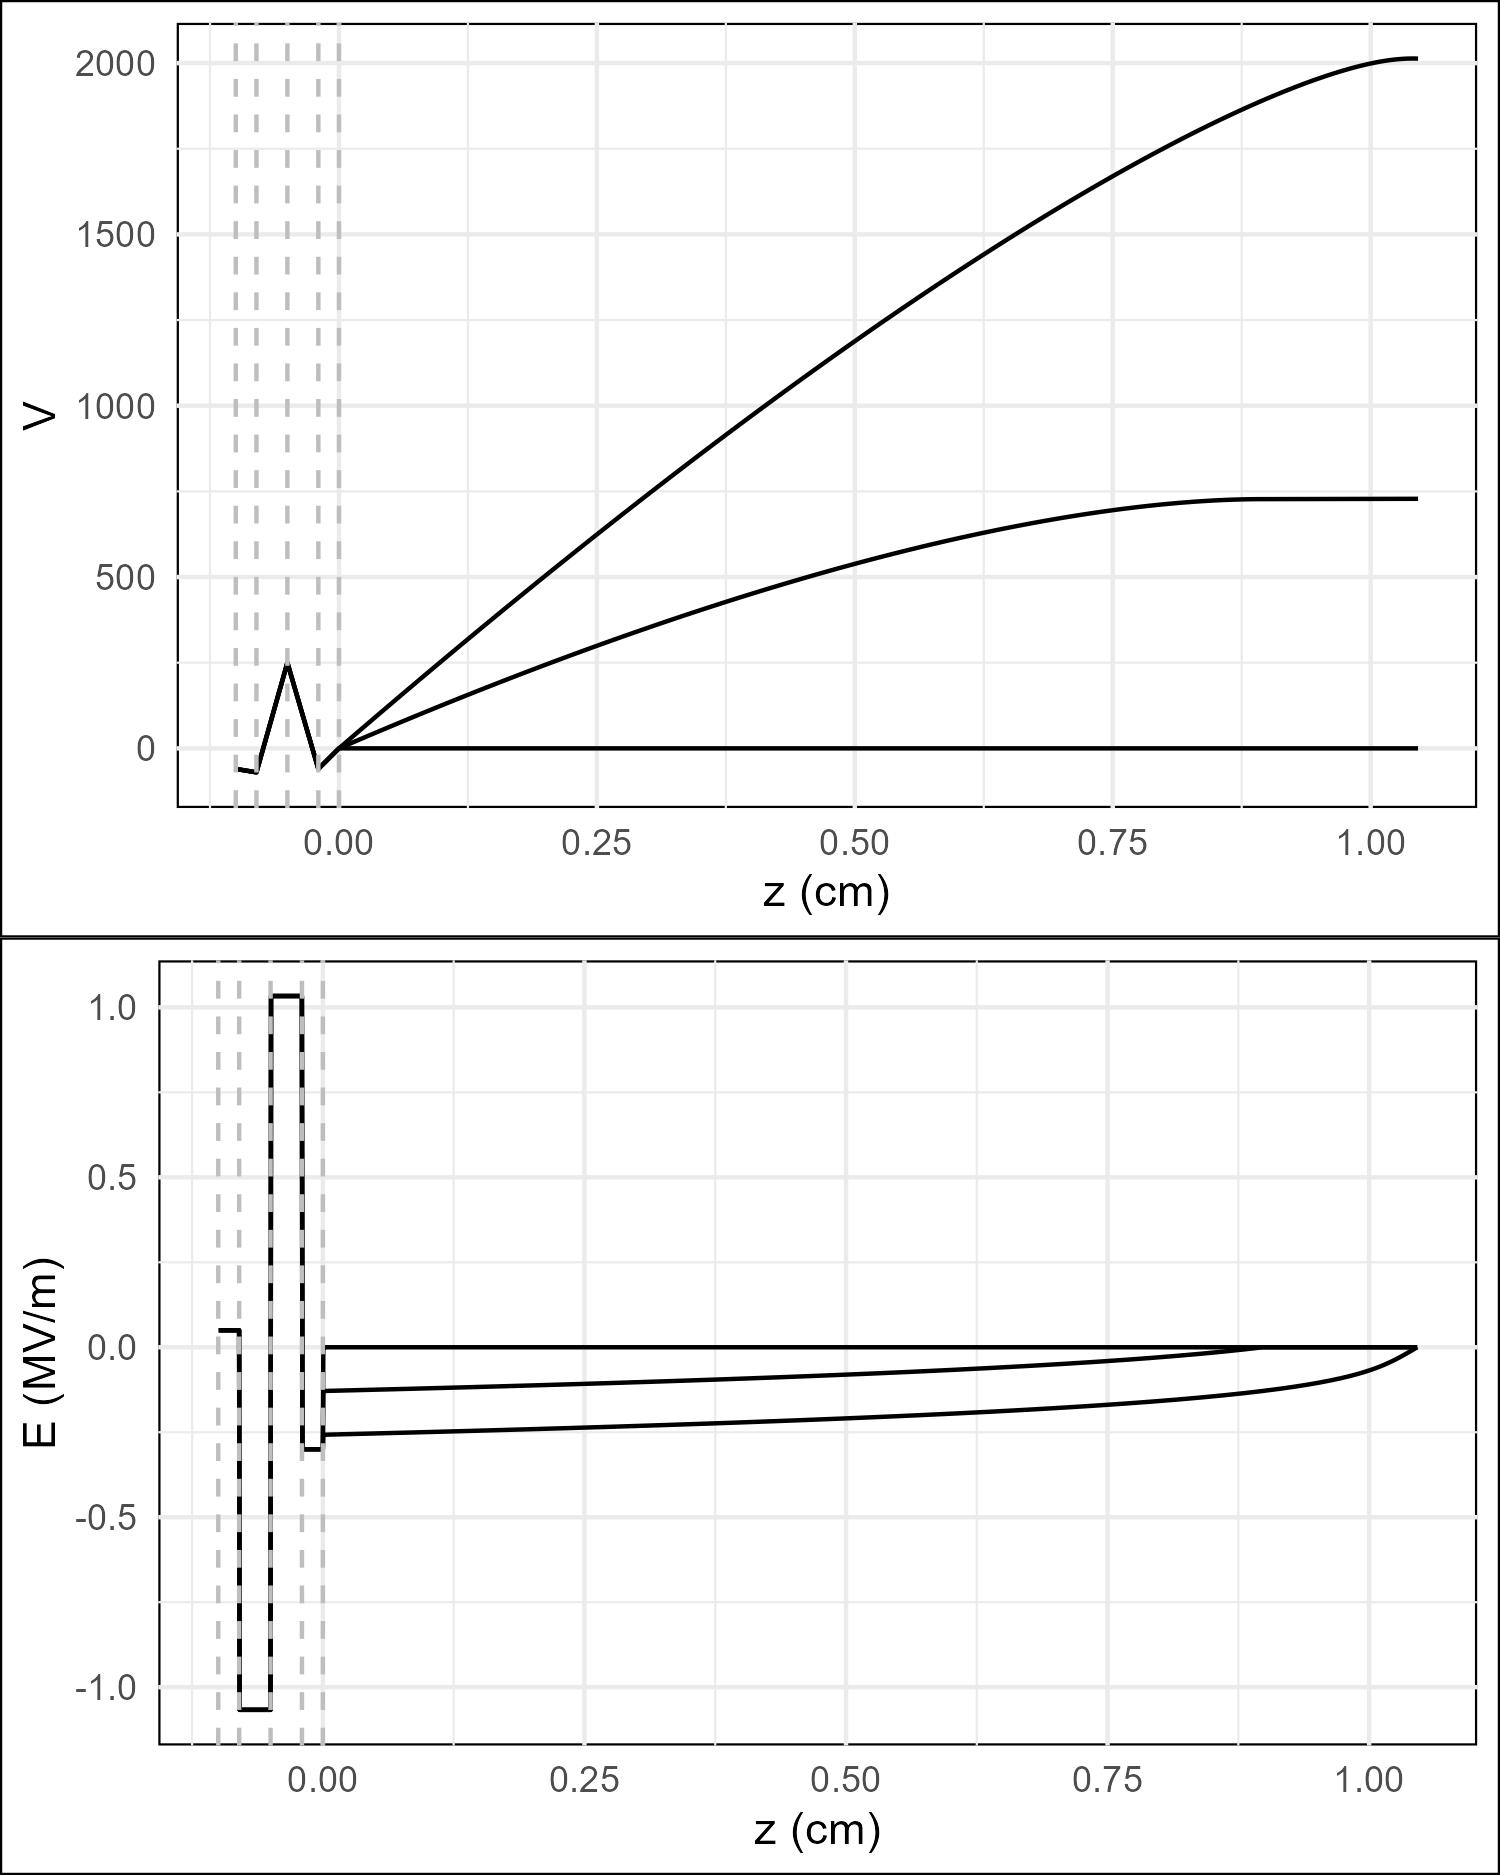
\includegraphics[width=0.45\textwidth]{Figures/VEz2Pa13.56MHz2kVStack2332.jpeg}
\caption{Space potential across a plasma sheath and RFEA grid stack (top) and corresponding electric field (bottom) for AC sheath solution with maximum voltage across the sheath of $2000$~V. Potential and field curves are shown for time $t=0$, $T/4$, and $T/2$. The sheath if fully expanded at $t=0$, at $z>1$~cm.}
\label{fig:ACpotentialField}
\end{figure}



\subsection{\label{IonTrajectory}Ion trajectory integration}
The ion trajectories under the force of the electric field in the sheath region and the RFEA region is integrated with a Runge-Kutta algorithm of fourth order. The integration time step is set to $dt=100$~ps. This time step is sufficiently small, i.e. an ion will have to reach a velocity of 1000~km/s to travel 100~$\mu$m (the thickness of an RFEA stack spacer) in time $dt$. The starting position for every ion is the sheath edge, $z=s_\text{Child Law}$ for the DC case, and the position of the fully expanded sheath in the AC case ($z=s_m$). All ions start with velocity equal to the Bohm velocity in the direction of the bounding electrode.
\begin{equation}
v_z = - v_\text{Bohm} = -\sqrt{\frac{e T_e}{M_\text{Ar}}}
\end{equation}
Where $M_\text{Ar}$ is the mass of the argon atom/ion. 

The ion flux is therefore, 
\begin{equation}
\Gamma_0 = e n_s v_\text{Bohm} 
\end{equation}

Fig.~\ref{fig:CollisionlessACtrajectory} shows a sample collisionless ion trajectory under the effect of the AC field of Fig.~\ref{fig:ACpotentialField}. Note the step increments in velocity corresponding to the modulation of the electric field in the sheath. Once in the RFEA region, the ion accelerates and decelerates according to the grid potentials. The ion in this case have enough energy to make it to the collector. 

\begin{figure}[htbp]
\centering
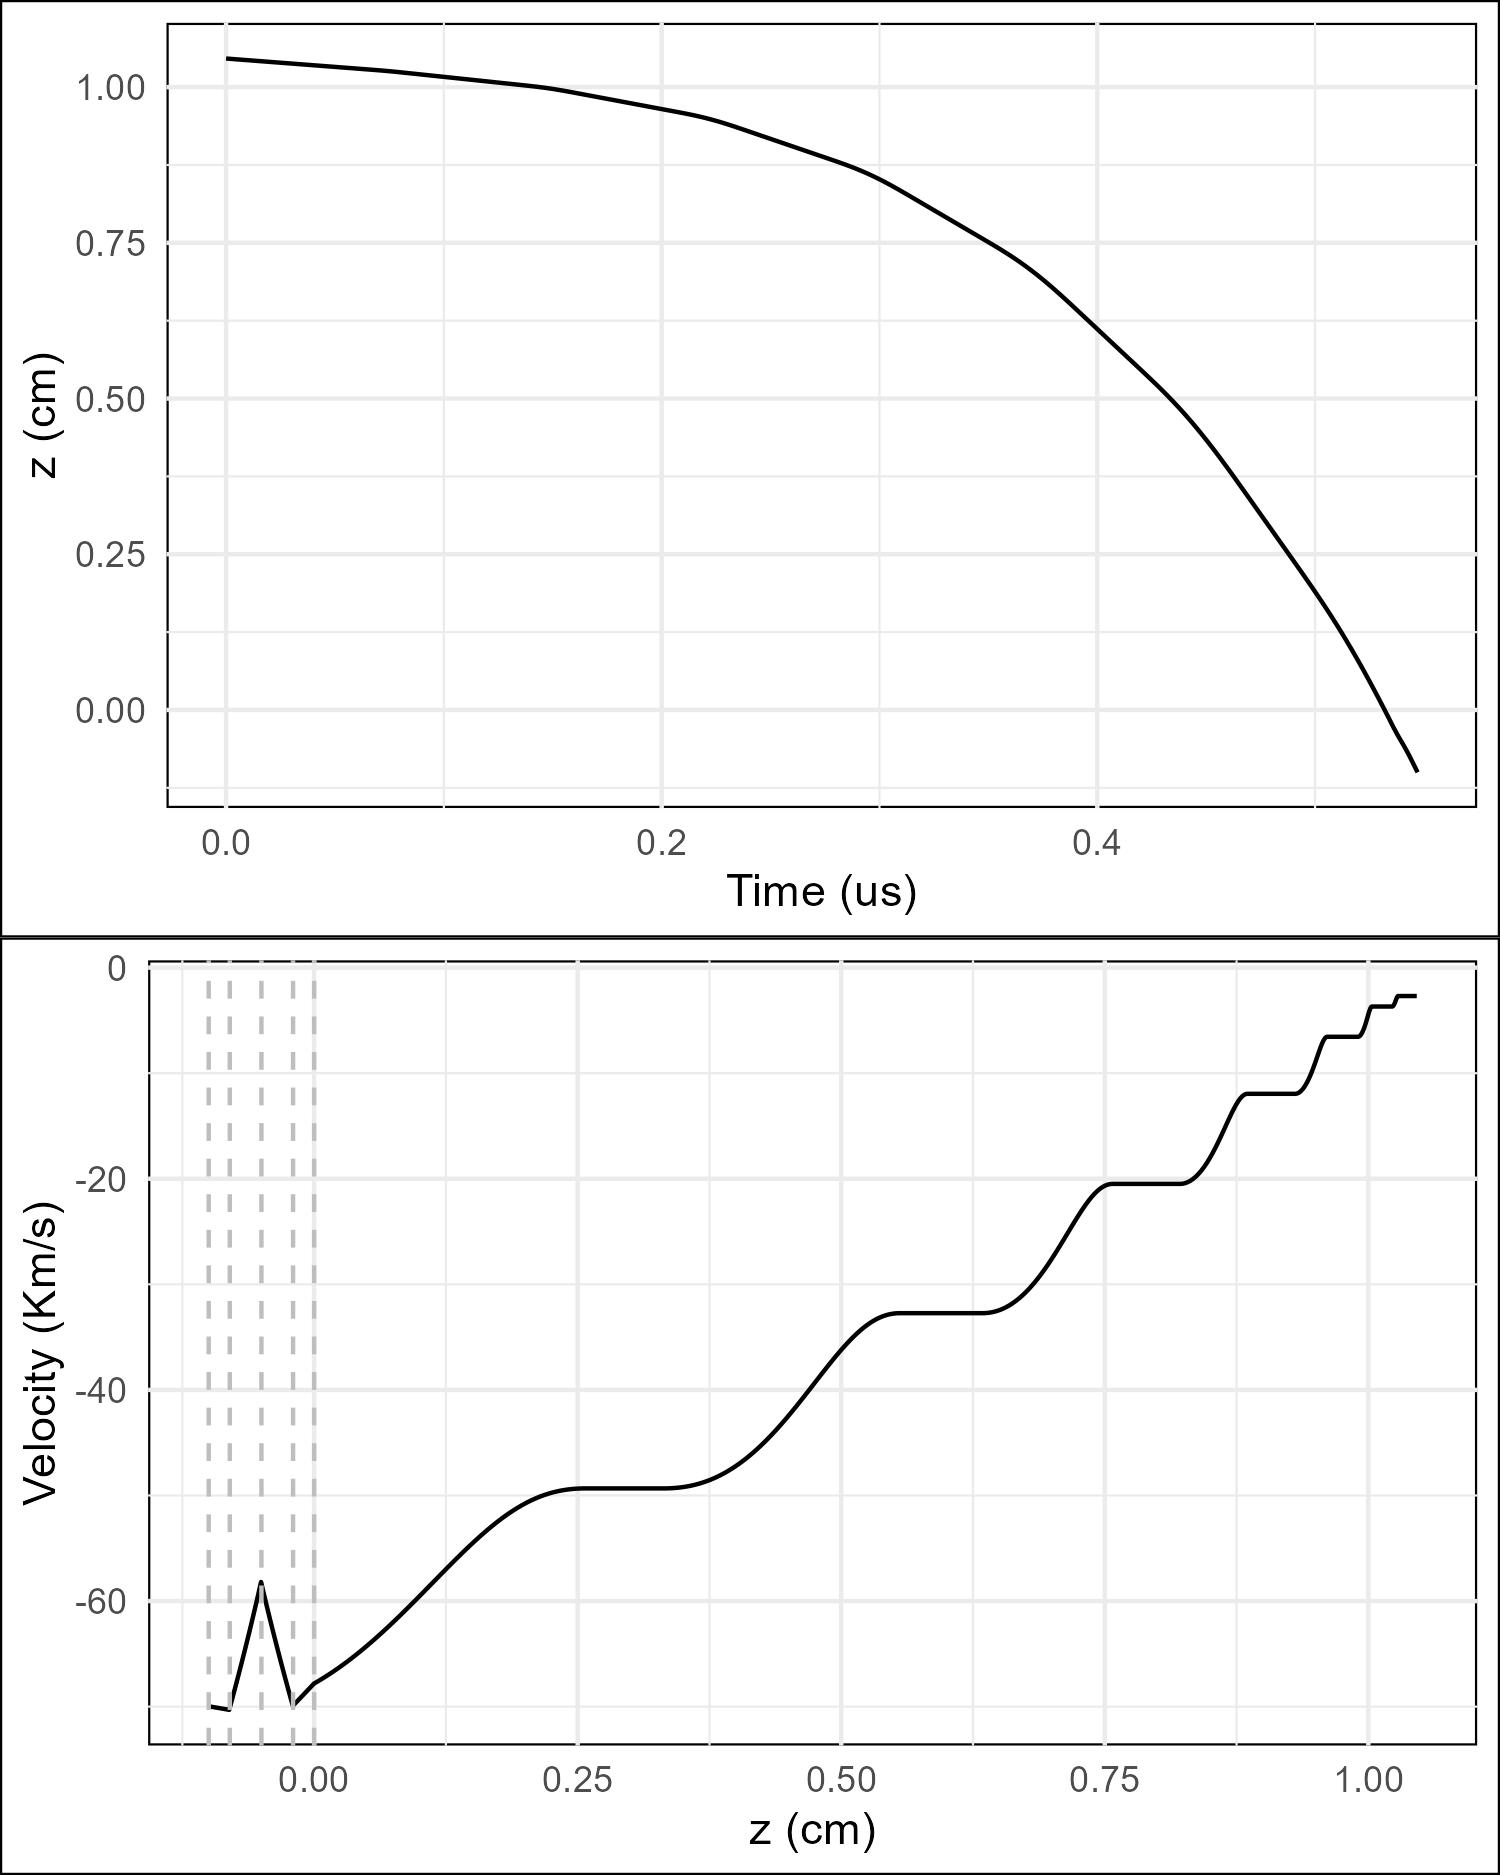
\includegraphics[width=0.45\textwidth]{Figures/ionTrajectory2Pa13.56MHz2kVStack2332_Collisionless.jpeg}
\caption{Collisionless sample trajectory of an argon ion from the plasma edge, through the plasma sheath and the RFEA for the AC sheath case of Fig.~\ref{fig:ACpotentialField}. The top plot shows the position of the ion in the z axis in time and the bottom plot shows the velocity of the ion in the z direction as a function of is position in z. }
\label{fig:CollisionlessACtrajectory}
\end{figure}



\subsection{\label{IonCollision}Collisions of ions with background gas}
Ion collisions are modelled using cross sections for two types of collisions
\begin{eqnarray}
\text{Ar}^+ + \text{Ar} &\rightarrow& \text{Ar}^+ + \text{Ar} \quad \text{(elastic)} \\
\text{Ar}^+ + \text{Ar} &\rightarrow& \text{Ar} + \text{Ar}^+ \quad \text{(charge exchange)} 
\end{eqnarray}
The cross sections for these two processes can be found in the LXCat database~\cite{LXCat}. The set for Ar ions was reported by Phelps~\cite{Phelps1994}. The isotropic collision cross section data set is used to model elastic collisions, and the backscattering collision cross section data is used to model charge exchange collisions. Except at very low energies, the charge exchange collision cross section is larger than the elastic collision cross section and therefore is the predominant collision process between argon ions and background argon gas (Fig.~\ref{fig:CrossSectionsArgon}). 

\begin{figure}[htbp]
\centering
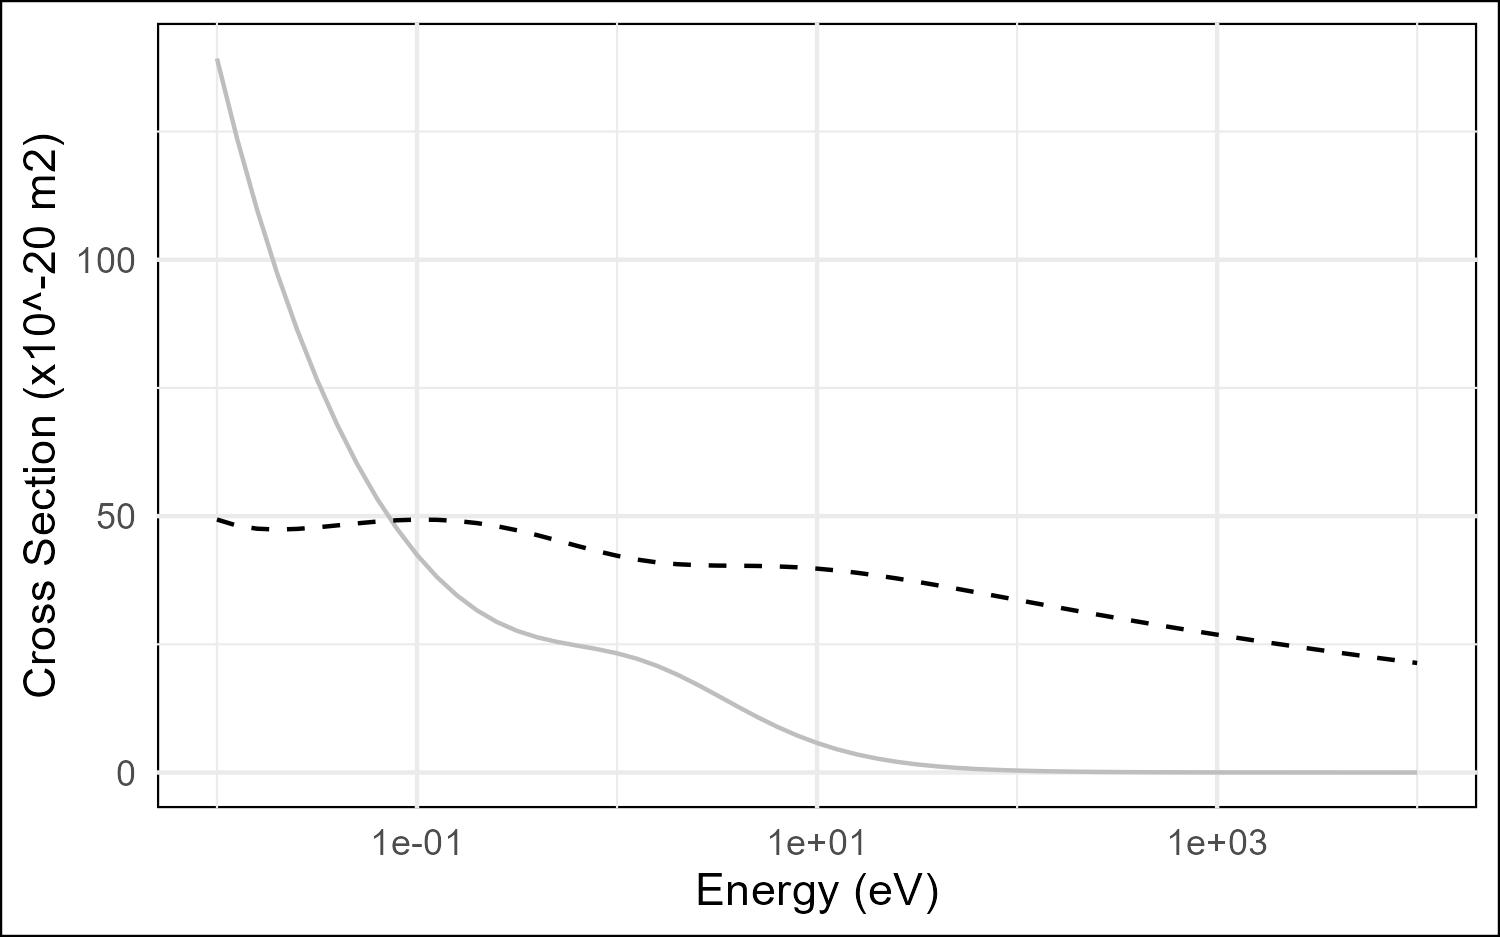
\includegraphics[width=0.45\textwidth]{Figures/CrossSections.jpg}
\caption{Cross sections for elastic (gray curve) and charge exchage collisions (dashed curve) for argon ion collisions with background argon gas~\cite{Phelps1994,LXCat}.}
\label{fig:CrossSectionsArgon}
\end{figure}

The probability of a collision at every time step is appoximated by
\begin{eqnarray}
P_{\text{col}} &=& \nu(\varepsilon) dt  \\
\nu(\varepsilon) &=& n_{\text{gas}} \sigma(\varepsilon) v_{\text{Ar}^+}
\end{eqnarray}
Where $\nu(\varepsilon)$ is the collision rate (s$^{-1}$), $n_{\text{gas}}$ is the density of neutral argon gas, $\sigma(\varepsilon) = \sigma_{\text{el}}(\varepsilon) + \sigma_{\text{cx}}(\varepsilon)$ is the total cross section (function of the ion energy), and $v_{\text{Ar}^+}$ is the velocity magnitude of the argon ion. A radom number is generated in the code every time step and if it is smaller than the probability of a collision then the ion velocity is modified according to one of the two processes. To determine which process to apply a second random number is generated and compared to 
\begin{equation}
P_{\text{el}} = \frac{\sigma_{\text{el}}(\varepsilon)}{\sigma_{\text{el}}(\varepsilon) + \sigma_{\text{cx}}(\varepsilon)}
\end{equation}
If the random number is smaller than $P_{\text{el}}$ then the collision is taken as elastic, otherwise it is charge exchange type. 

The elastic collision is processed as follows. First, a neutral argon atom is give a velocity vector in three-dimensional space  with magnitude equal to the mean average velocity (at 300~K) pointing in a random direction using random numbers to generate azimuth and polar angles. Second, the reference frame is changed from the laboratory refrence frame to the neutral argon atom reference frame. Third, the reference frame is rotated in the z-x plane to point in the direction that makes the argon ion parallel to the rotated z-axis. Fourth, a random number is used to generate a random scattering angle (between 0 and $\pi/2$) and to update the ion velocity vector. Fifth, the ion the reference frame is rotated back. Sixth, the reference frame is changed back to the laboratory refrence frame.

The charge exchange collision is processed as follows. First, a neutral argon atom is give a velocity vector in three-dimensional space  with magnitude equal to the mean average velocity (at 300~K) pointing in a random direction using random numbers to generate azimuth and polar angles. Second, this velocity is assigned to the argon ion.    

Fig.~\ref{fig:CollisionACtrajectory} shows the trajectory of an ion in an AC field (Fig.~\ref{fig:ACpotentialField}) with a collision event (charge exchange). The effect of the collision is the loss of the energy gained by the ion from the egde of the plasma up to the z position of the collision event. This type of collisions combined with the AC modulation of the sheath lead to complex ion energy distribution with multiple-peak structure~\cite{Wild1991}.

\begin{figure}[htbp]
\centering
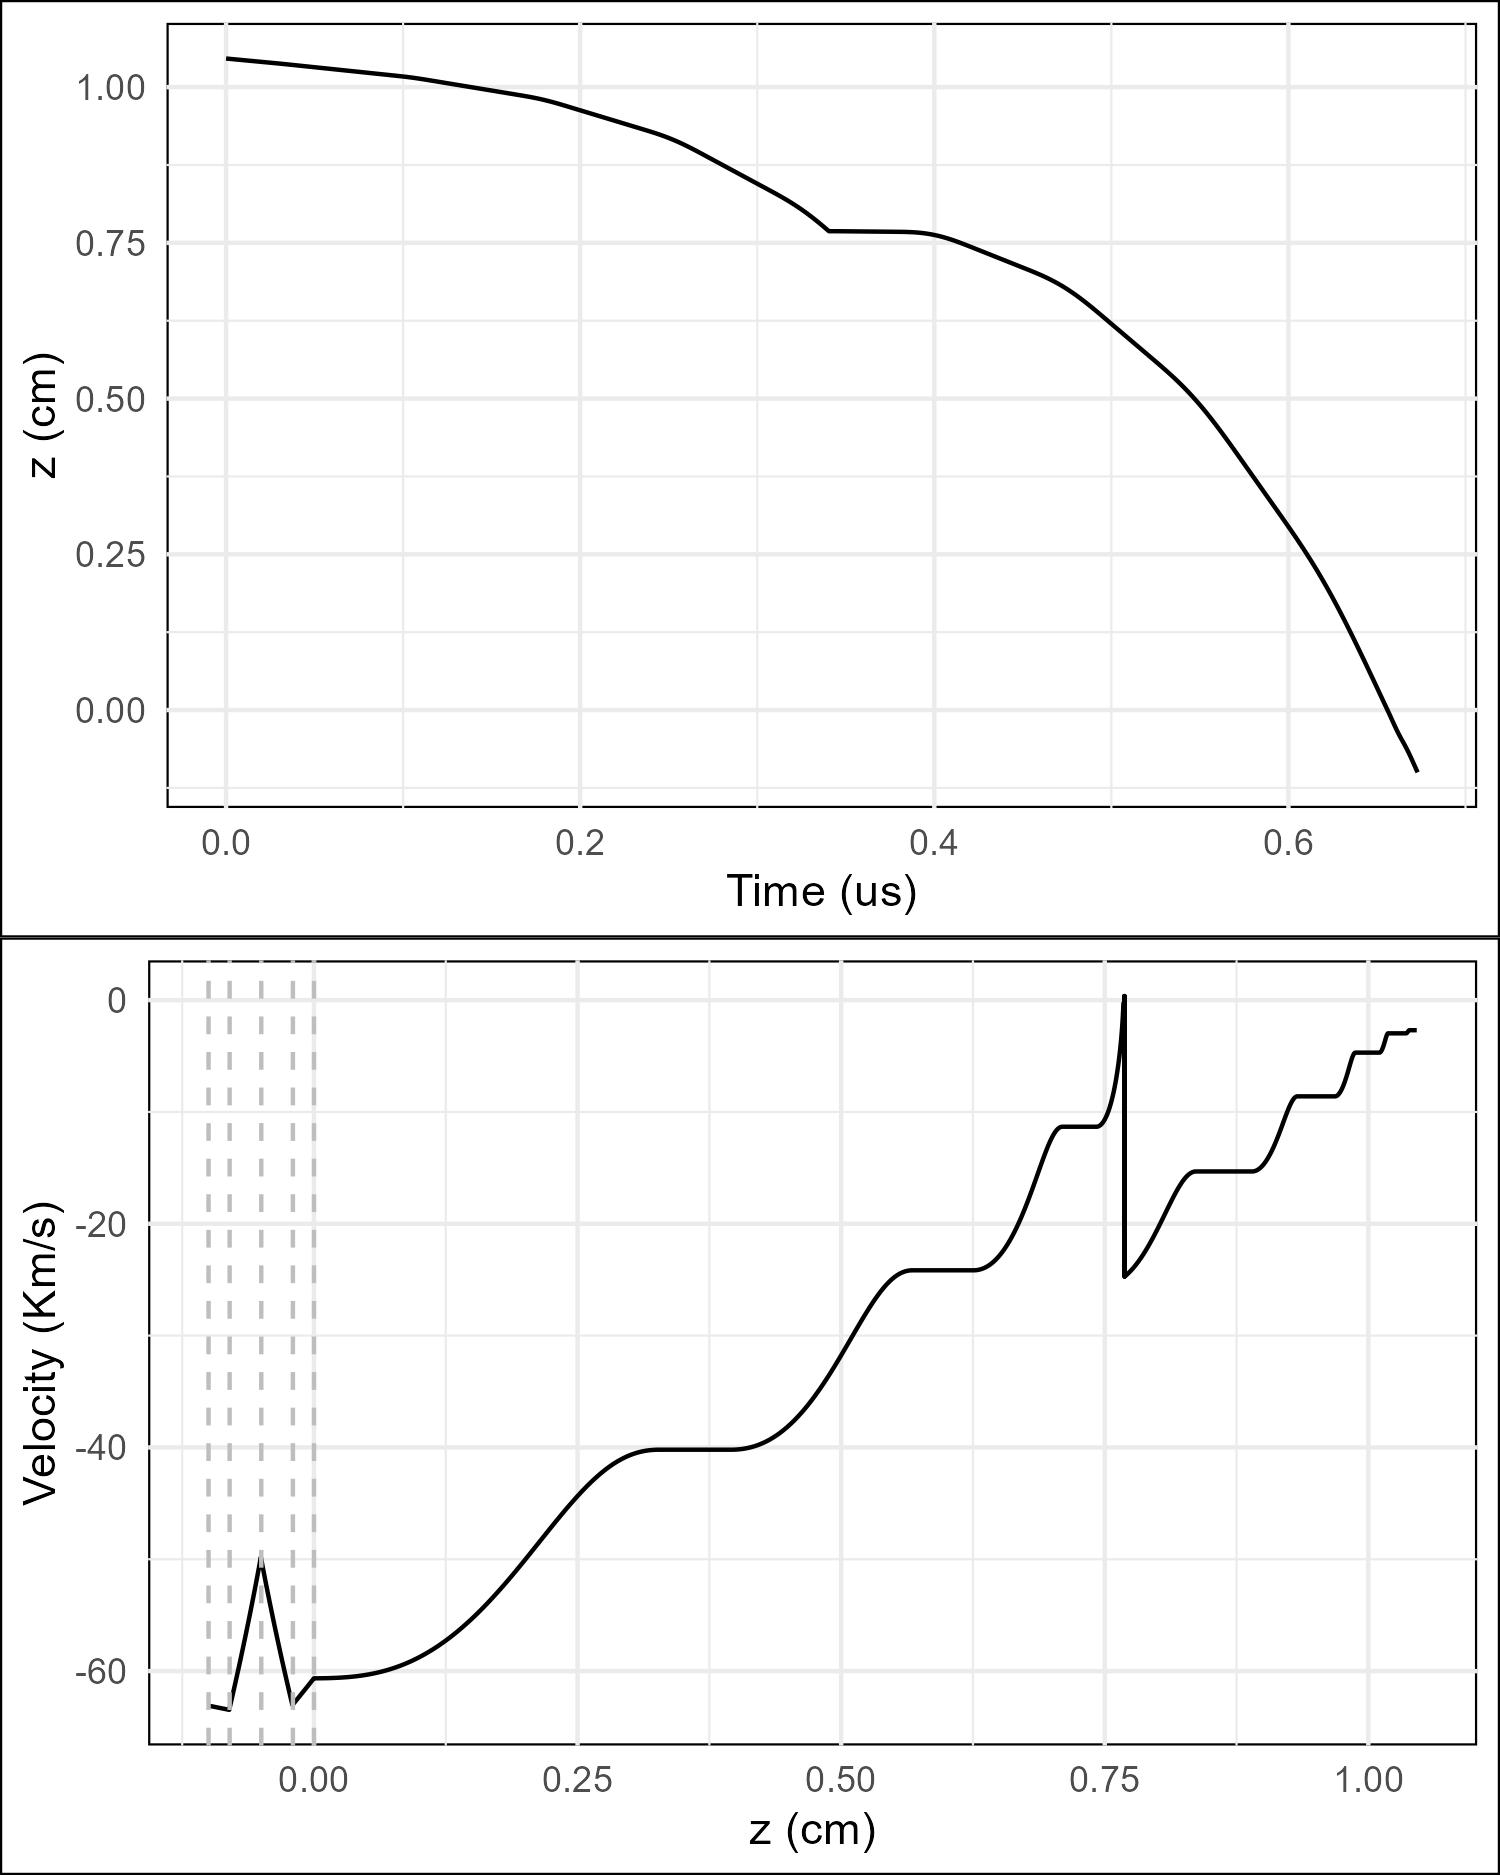
\includegraphics[width=0.45\textwidth]{Figures/ionTrajectory2Pa13.56MHz2kVStack2332.jpeg}
\caption{Sample trajectory of an argon ion including a collision event. The sheath is AC driven and the potential and field are those shown in Fig.~\ref{fig:ACpotentialField} }
\label{fig:CollisionACtrajectory}
\end{figure}



\nocite{*}
\bibliography{references}

\end{document}
